\documentclass[
    12pt,                % tamanho da fonte
    openright,           % capítulos começam sempre em página ímpar
    oneside,             % impressão só frente (use "twoside" se frente e verso)
    a4paper,             % papel A4
    brazil               % idioma principal
]{abntex2}

% Pacotes básicos
\usepackage[utf8]{inputenc}   % acentuação
\usepackage[T1]{fontenc}      % codificação da fonte
\usepackage{lmodern}          % usa fonte Latin Modern
\usepackage{microtype}        % melhora a justificação
\usepackage{graphicx}         % inserir figuras
\usepackage[alf]{abntex2cite}      % citações padrão ABNT
\usepackage{url}  
\usepackage{indentfirst}       % recuo no primeiro parágrafo
\usepackage{ragged2e}          % para justificação
\usepackage{amsmath} % para \text{} e outras paradas de equação
\usepackage{multirow} %para o multirow
\usepackage{float} % necessário para [H]
\usepackage{tikz} %desenho de diagramas
\usepackage{pgfplots}
\usepackage{tikz}
\usetikzlibrary{positioning, shapes.geometric, arrows.meta, arrows}



\pgfplotsset{compat=1.18} 




% Recuo e espaçamento entre parágrafos (ABNT)
\setlength{\parindent}{1.25cm} % recuo de 1,25 cm
\setlength{\parskip}{0.2cm}    % espaço entre parágrafos

% Informações do trabalho
\titulo{Título do seu TCC}
\autor{João Victor Sousa}
\local{Ilhéus - Bahia}
\data{2025}
\orientador{Otacílio José Pereira}
\instituicao{
  Universidade Estadual de Santa Cruz \par
  Curso de Graduação em Ciênca da Computação}
\tipotrabalho{Trabalho de Conclusão de Curso}
\preambulo{Trabalho apresentado ao Curso de Y da Universidade X como requisito parcial para obtenção do título de Bacharel.}

\begin{document}

% Capa e folha de rosto
\imprimircapa
\imprimirfolhaderosto*

% Resumo
\begin{resumo}
Escreva aqui o resumo do seu trabalho.  
Inclua objetivos, metodologia, resultados e conclusões.

\vspace{\onelineskip}
\noindent
\textbf{Palavras-chave}: palavra1. palavra2. palavra3.
\end{resumo}

% Sumário
\tableofcontents

%chapt* é um captulo sem numeração
\chapter*{Lista de Siglas} 
\begin{tabular}{ll}
AUC & Area Under Curve \\
RNN & Redes Neurais Recorrentes \\
CNN & Redes Neurais Convolucionais \\
LSTM & Long Short-Term Memory \\
AAMI & Association for the Advancement of Medical Instrumentation   \\
GRU & Gated Unit Recurrent \\
ECG & Eletrocardiograma \\
TP & Verdadeiro Positivo \\
FP & Falso Positivo \\
TN & Verdadeiro Negativo \\
FN & Falso Negativo \\
\end{tabular}


% Capítulos
\chapter{Introdução}
Texto da introdução.

\chapter{Fundamentação Teórica}

\section{ECG}

\subsection{O funcionamento do coração}

O coração é um órgão muscular composto por quatro câmaras que se contraem em sequência regular, bombeando o sangue de forma eficiente \cite{msd_ecg}. As contrações são controladas por correntes elétricas que percorrem o coração com precisão e velocidade regulada. 

O processo inicia no nódulo sinoatrial, localizado no átrio direito, que funciona como marcapasso natural do coração. A frequência cardíaca é determinada pela frequência de disparos desse nódulo, sendo modulada pelo sistema nervoso autônomo e por hormônios presentes na corrente sanguínea \cite{msd_ecg}. O sistema nervoso simpático aumenta a frequência cardíaca, enquanto o parassimpático, por meio do nervo vago, a reduz. Hormônios como a epinefrina (adrenalina) e norepinefrina (noradrenalina), produzidos pelo sistema simpático, também elevam a frequência cardíaca. Além disso, o hormônio tireoidiano liberado pela glândula da tireoide exerce influência na frequência cardíaca.

Em repouso, a frequência cardíaca em adultos varia entre 60 e 100 batimentos por minuto, sendo geralmente mais baixa em indivíduos jovens e em bom condicionamento físico \cite{msd_ecg}.

\subsection{Tipos de arritmia}

As arritmias podem ser classificadas de forma simplificada em três tipos principais:
\begin{itemize}
    \item Taquicardia: frequência excessivamente rápida;
    \item Bradicardia: frequência excessivamente lenta;
    \item Irregular: quando os impulsos percorrem o coração por vias irregulares.
\end{itemize}

\subsection{O batimento cardíaco}

O batimento cardíaco inicia-se no nódulo sinoatrial, cuja corrente elétrica atravessa o átrio direito e, em seguida, o átrio esquerdo, promovendo sua contração. O sangue é então impulsionado dos átrios para os ventrículos. A corrente elétrica passa pelo nódulo atrioventricular, único ponto de conexão entre átrios e ventrículos, que retarda o impulso, garantindo enchimento completo dos ventrículos. 

Em seguida, o impulso segue pelo feixe de His, que se divide em ramos para conduzir a corrente a cada ventrículo, permitindo sua ativação uniforme e subsequente contração, bombeando o sangue para o corpo \cite{msd_ecg}.

\subsection{O que é ECG?}

Segundo Cascino e Shea \cite{msd_ecg}, o eletrocardiograma (ECG) é um exame não invasivo que registra a atividade elétrica do coração. 
Ele é realizado pela colocação de eletrodos na pele do paciente, geralmente 12, chamados de derivações. 
Esses eletrodos registram tanto a direção quanto a magnitude da corrente elétrica. 

O registro resultante gera uma onda que reflete a atividade elétrica do coração. 
Cada etapa do ciclo cardíaco é representada na morfologia do traçado: 
a onda \textbf{P} corresponde à ativação dos átrios, 
o complexo \textbf{QRS} à ativação dos ventrículos 
e a onda \textbf{T} ao processo de repolarização ventricular.  

O ECG é uma ferramenta fundamental no diagnóstico de problemas cardíacos, 
permitindo identificar, por exemplo, episódios de infarto do miocárdio, 
oferta insuficiente de sangue e oxigênio ao coração (isquemia), 
hipertrofia das paredes cardíacas e diferentes tipos de arritmias.

\chapter{Metodologia}

Primeiramente, foi necessário definir qual banco de dados seria utilizado para o treinamento e a validação. Optou-se pelo \textit{MIT-BIH Arrhythmia Database} \cite{mitbih2005}, recomendado pela AAMI. O banco é composto por 58 registros de eletrocardiograma (ECG), cada um com 30 minutos de duração. Os 23 primeiros registros foram selecionados aleatoriamente a partir de um conjunto de 4000 gravações de 24 horas realizadas em pacientes ambulatoriais do Beth Israel Deaconess Medical Center. Os 25 registros restantes foram escolhidos de modo a incluir arritmias raras, mas clinicamente significativas.

Uma característica importante desse banco é a anotação de cada batimento cardíaco em torno do pico R, realizada por três cardiologistas independentes.

\section{Particionamento dos dados e classes}
\label{sec:particionamento}

Os dados foram particionados seguindo a estratégia inter-paciente proposta por Chazel et al. (apud \citeonline{silva2025}), na qual batimentos de um mesmo paciente não podem aparecer simultaneamente nos conjuntos de treinamento e validação. O objetivo é garantir a capacidade de generalização do modelo para diferentes pacientes. Além disso, conforme recomendado pela AAMI, registros de pacientes com marcapasso foram excluídos.  

Os registros 101, 106, 108, 109, 112, 114, 115, 116, 118, 119, 122, 124, 201, 203, 205, 207, 208, 209, 215, 220, 223 e 230 são normalmente chamados de DS1. Os demais (100, 103, 105, 111, 113, 117, 121, 123, 200, 202, 210, 212, 213, 214, 219, 221, 222, 228, 231, 232, 233 e 234) de DS2.

De acordo com a AAMI (apud \citeonline{silva2025}), são definidas cinco classes de arritmia: N, SVEB, VEB, F e Q, correspondentes a batimento normal, batimento supraventricular ectópico, batimento ventricular ectópico, fusão de batimento ventricular e normal e batimento não classificado, respectivamente. A Tabela~\ref{tab:particionamento} apresenta a distribuição dessas classes no conjunto de dados.

\begin{table}[htb]
\centering
\caption{Particionamento inter-paciente proposto por Chazel et al.}
\label{tab:particionamento}
\begin{tabular}{|l|c|c|c|c|c|c|}
\hline
Conjunto & N & SVEB & VEB & F & Q & Total \\ \hline
DS1 & 45 866 & 944 & 3 788 & 415 & 8 & 51 021 \\ \hline
DS2 & 44 259 & 1 837 & 3 221 & 388 & 7 & 49 712 \\ \hline
Total & 90 125 & 2 781 & 7 009 & 803 & 15 & 100 733 \\ \hline
\end{tabular}
\legend{Fonte: Adaptado de Silva et al. (2025).}
\end{table}

O conjunto DS1 foi então subdividido em treinamento e validação por meio de validação cruzada, inicialmente com duas partições (dois \textit{folds}) e, posteriormente, com cinco partições (cinco \textit{folds}) nos modelos finais.  

É importante ressaltar que o MIT-BIH detalha muito outros tipos de batimentos. Essas cinco classes são uma proposta da AAMI, feita a partir do agrupamento desses tipos.
Uma lista das anotações pode ser encontrada em \cite{physionet_annotations}. O mapeamento entre os tipos descritos originalmente e as cinco classes foi feito da seguinte maneira:

\begin{table}[H]
\centering
\caption{Mapeamento das anotações originais do MIT-BIH para as classes AAMI.}
\label{tab:mapeamento_classes}
\begin{tabular}{ll}
\hline
\textbf{Anotação Original} & \textbf{Classe AAMI} \\
\hline
N, e, j, L, R & N (Normal) \\
A, a, J, S & S (Supraventricular) \\
V, E & V (Ventricular) \\
F, f & F (Fusão) \\
Q, ?, / & Q (Desconhecida) \\
\hline
\end{tabular}
\end{table}


Considerando o desbalanceamento dos dados e visando maior simplicidade, adotou-se a classificação binária; onde a classe positiva corresponde a arritmia ventricular e a negativa ao batimento normal.

A arritmia ventricular é o tipo arrítmico mais prevalente no MIT-BIH e apresenta uma morfologia marcante. Ela é composta dos tipos arrítmicos: contração prematura
contração ventricular prematura (classe V) e batimento de escape ventricular (classe E).


\section{Métricas}
\label{sec:metricas}

As métricas utilizadas para avaliar o desempenho dos modelos foram: sensibilidade, precisão, acurácia, \textit{F1-score} e AUC (\textit{Area Under the Curve}).  

A sensibilidade representa a capacidade do modelo em identificar corretamente as classes positivas, isto é, os batimentos arrítmicos. Sua equação é dada por:

\begin{equation}
\text{Sensibilidade} = \frac{TP}{TP + FN}
\end{equation}

em que $TP$ são os verdadeiros positivos e $FN$ os falsos negativos.  

A precisão, por sua vez, indica a proporção de batimentos classificados como arrítmicos que realmente pertencem a essa classe:

\begin{equation}
\text{Precisão} = \frac{TP}{TP + FP}
\end{equation}

onde $FP$ representa os falsos positivos. Precisão e sensibilidade estão relacionadas por um \textit{trade-off}. No contexto médico, prioriza-se elevada sensibilidade, ainda que à custa de menor precisão, uma vez que falsos negativos são mais prejudiciais que falsos positivos.  

O \textit{F1-score} é a média harmônica entre precisão e sensibilidade, buscando um equilíbrio entre ambas:

\begin{equation}
\text{\textit{F1-score}} = \frac{2 \cdot \text{Precisão} \cdot \text{Sensibilidade}}{\text{Precisão} + \text{Sensibilidade}}
\end{equation}

A acurácia corresponde ao acerto global do modelo, considerando tanto as classes positivas quanto as negativas:

\begin{equation}
\text{Acurácia} = \frac{TP + TN}{TP + TN + FP + FN}
\end{equation}

A AUC mede a capacidade do modelo em separar as classes positivas das negativas, variando entre 0 e 1. Valores próximos de 1 indicam separação perfeita, enquanto 0,5 corresponde a um modelo com desempenho equivalente ao acaso. 

Essa métrica é calculada a partir da área sob a curva ROC, ilustrada na Figura~\ref{fig:roc}.


\begin{figure}[H]
    \centering
    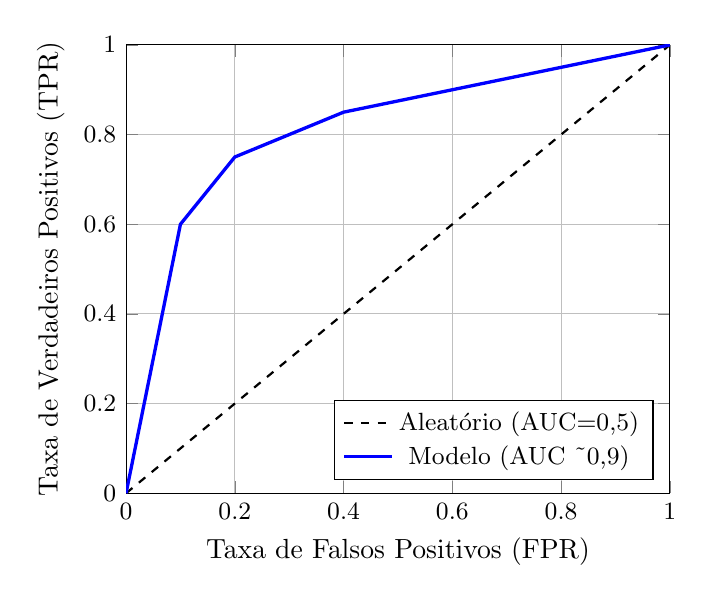
\begin{tikzpicture}
        \begin{axis}[
            width=0.7\textwidth,
            height=0.6\textwidth,
            grid=both,
            xlabel={Taxa de Falsos Positivos (FPR)},
            ylabel={Taxa de Verdadeiros Positivos (TPR)},
            xmin=0, xmax=1,
            ymin=0, ymax=1,
            legend pos=south east,
            legend style={font=\small},
            tick label style={font=\small}
        ]

        % Linha do classificador aleatório
        \addplot[domain=0:1, dashed, thick, color=black] {x};
        \addlegendentry{Aleatório (AUC=0,5)}

        % Curva ROC simulada
        \addplot[color=blue, very thick] coordinates {
            (0,0)
            (0.1,0.6)
            (0.2,0.75)
            (0.4,0.85)
            (0.6,0.9)
            (0.8,0.95)
            (1,1)
        };
        \addlegendentry{Modelo (AUC \textasciitilde 0,9)}

        \end{axis}
    \end{tikzpicture}
    \caption{Exemplo de curva ROC: comparação entre modelo aleatório e modelo com bom desempenho.}
    \label{fig:roc}
\end{figure}

Já a curva PR, Precisão vs \textit{Recall}, ilustrada abaixo:


\pgfplotsset{compat=1.18}

\begin{figure}[H]
    \centering
    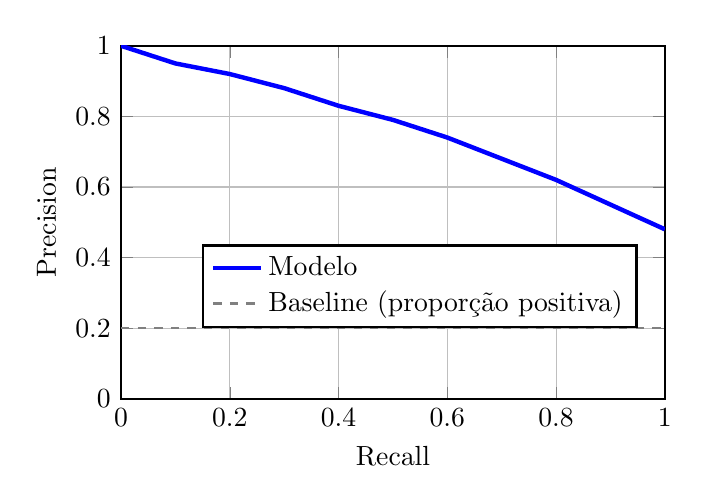
\begin{tikzpicture}
        \begin{axis}[
            width=0.7\textwidth,
            height=0.5\textwidth,
            xlabel={Recall},
            ylabel={Precision},
            xmin=0, xmax=1,
            ymin=0, ymax=1,
            grid=major,
            legend style={at={(0.95,0.2)},anchor=south east},
            legend cell align={left},
            thick
        ]
        % Curva principal (exemplo genérico)
        \addplot[color=blue, ultra thick] coordinates {
            (0.0,1.0)
            (0.1,0.95)
            (0.2,0.92)
            (0.3,0.88)
            (0.4,0.83)
            (0.5,0.79)
            (0.6,0.74)
            (0.7,0.68)
            (0.8,0.62)
            (0.9,0.55)
            (1.0,0.48)
        };
        \addlegendentry{Modelo}

        % Linha base (baseline)
        \addplot[dashed, color=gray] coordinates {
            (0,0.2) (1,0.2)
        };
        \addlegendentry{Baseline (proporção positiva)}
        \end{axis}
    \end{tikzpicture}
    \caption{Curva Precision–Recall genérica .}
    \label{fig:pr_curve_nv}
\end{figure}


Na figura \ref{fig:pr_curve_nv} representa uma curva PR genérica, a curva mostra a precisão em função do \textit{recall}. Como ilustrado,
conforme aumenta-se o \textit{recall}, há uma diminuição da precisão e vice-versa; representado o \textit{trade-off}. O AP é a área do gráfico; quanto
maior, melhor. Um modelo aleatório teria um AP igual a frequência da classe positiva.

A matriz de confusão, por fim, fornece uma representação tabular dos acertos e erros do modelo, como exemplificado na Tabela~\ref{tab:matriz_confusao}.

\begin{table}[H]
\centering
\caption{Exemplo de matriz de confusão binária}
\label{tab:matriz_confusao}
\begin{tabular}{|c|c|c|}
\hline
\multirow{2}{*}{\textbf{Classe Verdadeira}} & \multicolumn{2}{c|}{\textbf{Classe Predita}} \\ \cline{2-3} 
 & Positiva & Negativa \\ \hline
Positiva & TP & FN \\ \hline
Negativa & FP & TN \\ \hline
\end{tabular}
\legend{Fonte: Elaborado pelo autor.}
\end{table}

Essas métricas em conjunto permitem avaliar não apenas a proporção global de acertos, mas também a capacidade do modelo em detectar corretamente arritmias, aspecto essencial em aplicações médicas.

\section{Tipos de redes usadas}
\label{sec:tipo_redes}

Inicialmente, foram escolhidas redes neurais recorrentes (RNNs) e seus subtipos, como LSTM e GRU. Segundo \citeonline{james2023}, esse tipo de rede apresenta grande potencial para lidar com dados sequenciais, como no processamento de linguagem natural, previsão de preços e outros tipos de séries temporais. Como o componente temporal é relevante para o diagnóstico das arritmias, optou-se por esse tipo de modelo.

Além das RNNs, foram utilizadas redes neurais convolucionais (CNNs), conhecidas por sua habilidade em reconhecer padrões em diferentes domínios \citeonline{james2023}. Em particular, CNNs unidimensionais (1D-CNNs) têm se mostrado eficazes na análise de sinais fisiológicos, sendo amplamente aplicadas à classificação de ECG \cite{narotamo2024}.

A motivação para essa combinação está na complementaridade entre os modelos: enquanto as RNNs são eficazes na captura de dependências temporais, as CNNs se destacam na identificação de características morfológicas do sinal.

\section{Pré-processamento e entrada para os modelos}
\label{sec:pre_process}

Antes de usar o sinal do ECG como entrada, ele precisou passar por uma etapa de pré-processamento que consistiu em uma limpeza de ruídos e segmentação.
Para a diminuição do ruído, foi utilizando um filtro passa-alta de ordem 5 de 0,5 hz, seguido por uma filtragem de linha de energia de 60hz. 
Isso foi importante para remover ruídos musculares e ruídos oriundos da alimentação dos aparelhos. 

Em seguida, os batimentos foram segmentados em batimentos individuais. Nas duas etapas foram utilizadas a biblioteca NeuroKit2 \cite{Makowski2021neurokit}

O objetivo do trabalho é a classificação de batimentos cardíacos em duas classes: normais e arritmia ventricular. 
Para isso, os modelos recebem uma sequência de 16 batimentos e realizam a classificação do último batimento da sequência. 
Cada sequência é composta exclusivamente por batimentos de um único paciente

Tanto as CNNs quanto as RNNs recebem como entrada uma matriz tridimensional com a seguinte estrutura: $(\text{tamanho do batch}, \text{tamanho da sequência}, \text{número de features})$.

Para otimização do processo de treinamento, foram utilizados os mecanismos de \textit{early stopping} e \textit{reduce on plateau}, responsáveis por limitar o número de épocas e ajustar dinamicamente a taxa de aprendizagem, respectivamente.

\section{Arquiteturas}
\label{sec:modelos}

Foram testadas dois tipos de arquiteturas, uma é o uso de RNNs puras e a outra é uma arquitetura híbrida com CNNs. 

A primeira arquitetura de pura é composta por três camadas de GRUs com 256 unidades ocultas. Essa arquitetura foi utilizada em \citeonline{narotamo2024}, onde obteve o melhor desempenho. 
A diferença é que nesse trabalho, além da rede receber o sinal do ECG, ela também recebeu os intervalos RRs pré e pós:


\begin{figure}[H]
  \centering
  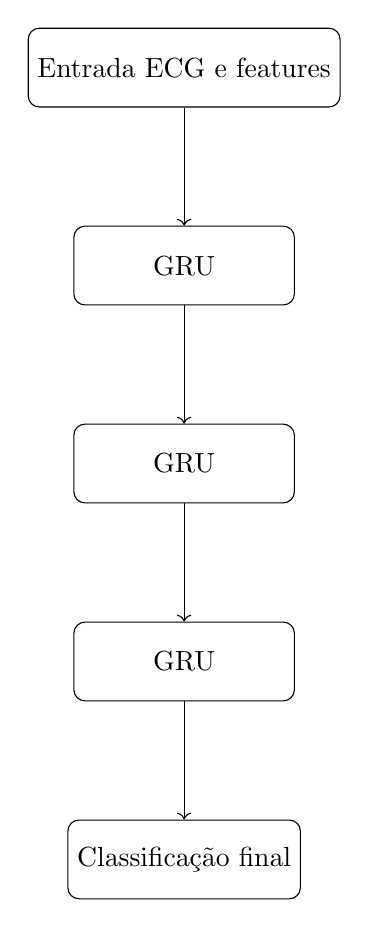
\begin{tikzpicture}[node distance=1.5cm, every node/.style={draw, rounded corners, minimum width=2.8cm, minimum height=1cm, align=center}]

\node (input){Entrada ECG e features};
\node [below=of input](gru_1){GRU};
\node [below=of gru_1](gru_2){GRU};
\node [below=of gru_2](gru_3){GRU};
\node [below=of gru_3](saida){Classificação final};

%conexões:

\draw[->](input) -- (gru_1);
\draw[->](gru_1) -- (gru_2);
\draw[->](gru_2) -- (gru_3);
\draw[->](gru_3) -- (saida);
\end{tikzpicture}
 % insere o tikzpicture puro
  \caption{Arquitetura híbrida CNN+GRU.}
  \label{fig:gru_pura}
\end{figure}

A segunda rede é uma híbrida de CNN com GRU:

\begin{figure}[H]
  \centering
  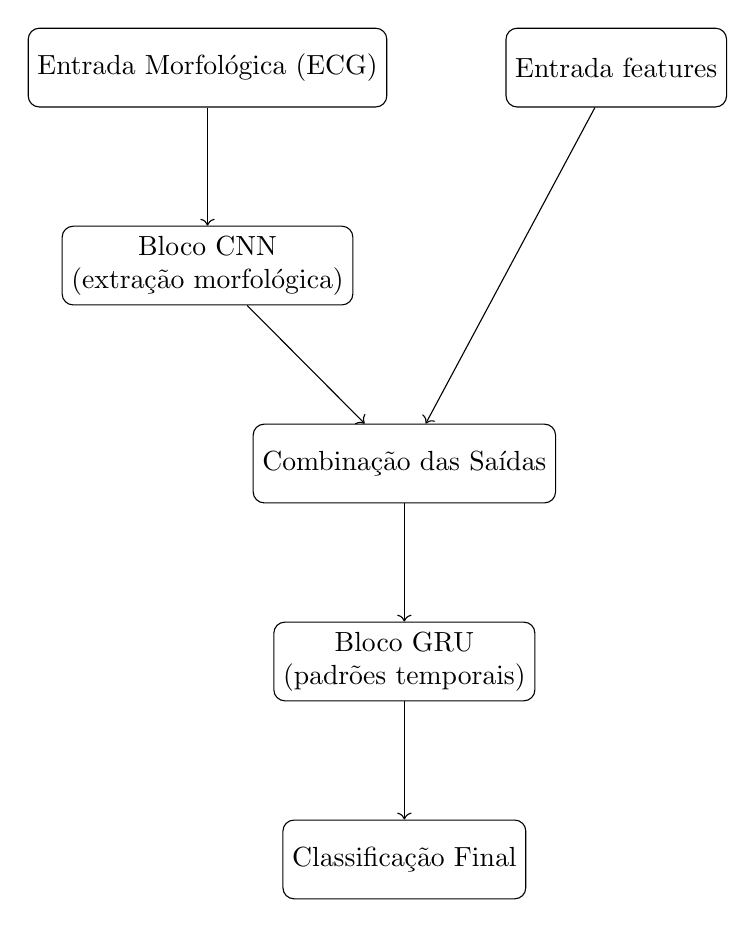
\begin{tikzpicture}[node distance=1.5cm, every node/.style={draw, rounded corners, minimum width=2.8cm, minimum height=1cm, align=center}]

% Entradas
\node (morf) {Entrada Morfológica (ECG)};
\node[right=of morf] (ritmo) {Entrada features};

%blocos de redes neurais:
\node[below=1.5cm of morf] (cnn) {Bloco CNN \\ (extração morfológica)};

% Combinação
\node[below=1.5cm of cnn, xshift=2.5cm] (fusion) {Combinação das Saídas};

% Bloco RNN
\node[below=of fusion] (rnn) {Bloco GRU \\ (padrões temporais)};

%saída
\node[below=of rnn] (saida) {Classificação Final};

%conexões
\draw[->](morf) -- (cnn);
\draw[->](cnn) -- ++ (fusion);
\draw[->](ritmo) -- ++ (fusion);
\draw[->](fusion) -- (rnn);
\draw[->](rnn) -- (saida);

\end{tikzpicture}

 % insere o tikzpicture puro
  \caption{Arquitetura híbrida CNN+GRU.}
  \label{fig:cnn_gru}
\end{figure}

O bloco de CNN precisou ser aplicado em cada batimento dentro da sequência. Trata-se de duas camadas de CNN com 32 e 64 filtros respectivamente e cada 
uma seguida por uma camada de \textit{batch normalization} e \textit{global max pooling} para evitar sobre ajuste e reduzir as \textit{features} respectivamente.

Enquanto que a rede da figura \ref{fig:gru_pura} recebeu o ECG concatenado com as \textit{features}, a rede híbrida as recebeu separadas, sendo conectadas após o processamento
das CNNs.

\chapter{Resultados e discussões}

\section{Resultados do modelo GRU}

A seguir, os resultados alcançados pelo modelo descrita em \ref{fig:gru_pura}, proposta por \cite{narotamo2024}:

\begin{table}[H]
\centering
\caption{Resultados do GRU (\textit{N} vs. \textit{V}) na validação}
\label{tab:resultado_cv_gru_validacao}
\begin{tabular}{lcc}
\hline
\textbf{Métrica} & \textbf{Média} & \textbf{Desvio Padrão} \\
\hline
Precisão & 0.8515 & 0.1825 \\
\textit{Recall} & 0.8039  & 0.0795 \\
\textit{F1-Score} & 0.8060 & 0.0760 \\
Acurácia & 0.9640 & 0.0278 \\
\hline
\end{tabular}
\end{table}

Na tabela \ref{tab:resultado_cv_gru_validacao}, tem-se as métricas médias com seus respectvios desvio padrão na \textit{cross-validação} de cinco \textit{folds}.
Os resultados indicam que o modelo achou aproximadamente 80\% dos casos positivos, com um desvio padrão relativamente baixo, indicando boa estabilidade.
Além disso, a precisão do modelo foi maior que seu \textit{recall}, indicando um perfil mais conservador na classificação. 

A seguir os resultados no treino:

\begin{table}[H]
\centering
\caption{Resultados do GRU (\textit{N} vs. \textit{V}) no treino}
\label{tab:resultado_cv_gru_treino}
\begin{tabular}{lcc}
\hline
\textbf{Métrica} & \textbf{Média} & \textbf{Desvio Padrão} \\
\hline
Precisão & 0.9872 & 0.0121 \\
Revocação & 0.9782 & 0.0150 \\
F1-Score & 0.9827 & 0.0134 \\
Acurácia & 0.9969 & 0.0024 \\
\hline
\end{tabular}
\end{table}

Pelos resultados da tabela \ref{tab:resultado_cv_gru_treino}, há uma evidência de sobreaguaste; isto é, o modelo apresenta uma falha em sua capacidade
de generalização. Durante o treino de um modelo de aprendizado de máquina, busca-se a partir de uma amostra da população estimar uma curva que melhor
se encaixa na população. Modelos flexíveis como uma rede neural tem uma grande capacidade de se ajustar a essa amostra e, caso ela seja pequena, por exemplo,
o modelo pode acabar aprendendo as particularidades da amostra ao invés de padrões generalizáveis. 

No caso do MIT-BIH; o desbalanceamento junto com as diferenças entre os batimentos de cada paciente pode ter causado esse sobre-ajuste.

A seguir, a matriz de confusão no melhor e pior \textit{fold} respectivamente:

\begin{figure}[H]
  \centering
   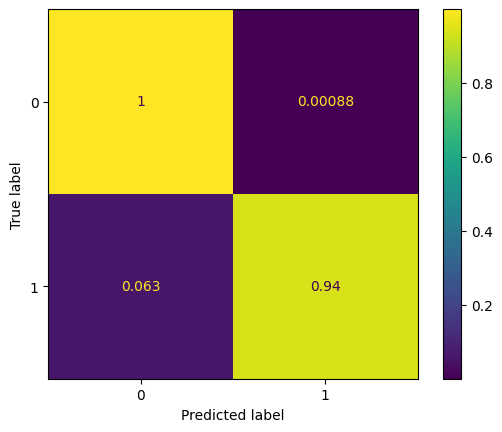
\includegraphics[width=0.7\textwidth]{figuras/modelos_resultados/matriz_confusao_melhor_fold_gru.png} % insere o tikzpicture puro
  \caption{Matriz de confusão do modelo \ref{fig:gru_pura} em seu melhor \textit{fold}}
  \label{fig:matriz_confusao_melhor_fold_gru}
\end{figure}

Pel figura \ref{fig:ap_gru_melhor_fold}, no melhor \textit{fold}, o modelo achou 96\% das arritmias. Porém no pior, como pode ser visto
na figura \ref{fig:ap_gru_pior_fold}, o modelo só conseguiu achar 76\% das classes positivas

\begin{figure}[H]
  \centering
   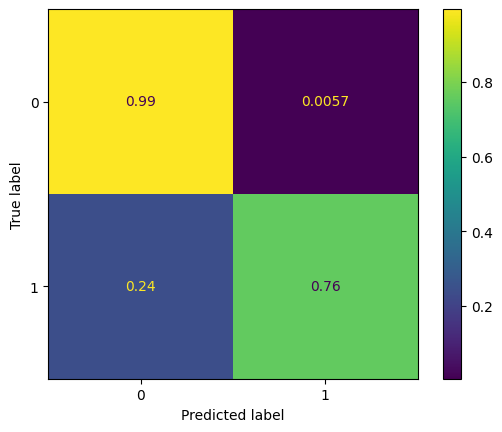
\includegraphics[width=0.7\textwidth]{figuras/modelos_resultados/matriz_confusao_pior_fold_gru.png} % insere o tikzpicture puro
  \caption{Matriz de confusão do modelo \ref{fig:gru_pura} em seu pior \textit{fold}}
  \label{fig:matriz_confusao_pior_fold_gru}
\end{figure}

As duas figuras ilustram como o modelo conseguiu aprender melhor a classe negativa do que a classe positiva; evidenciado pelo fato dele confundir
muito menos negativo com positivo do que o contrário. Um resultado esperado devido a essa ser a classe dominante em todos os \textit{folds}.

A seguir a curva ROC no melhor \textit{fold}:


\begin{figure}[H]
  \centering
   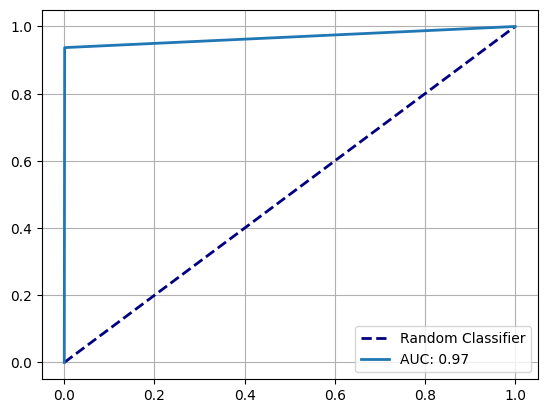
\includegraphics[width=0.7\textwidth]{figuras/modelos_resultados/roc_gru_melhor_fold.png} % insere o tikzpicture puro
  \caption{Curva \textit{ROC} modelo \ref{fig:gru_pura} em seu melhor \textit{fold}}
  \label{fig:roc_melhor_fold_gru}
\end{figure}

Considerando que o \textit{baseline}, um classificador aleatório, tem um \textit{ROC} de 0.5, o melhor foi significantemente melhor.

\begin{figure}[H]
  \centering
   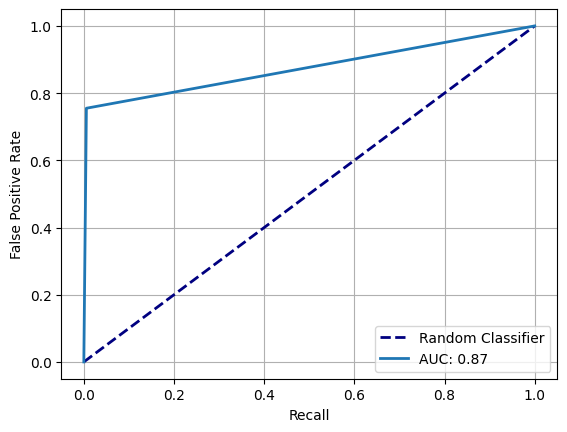
\includegraphics[width=0.7\textwidth]{figuras/modelos_resultados/roc_gru_pior_fold.png} % insere o tikzpicture puro
  \caption{Curva \textit{ROC} do modelo \ref{fig:gru_pura} em seu melhor \textit{fold}}
  \label{fig:roc_pior_fold_gru}
\end{figure}

No pior fold, \ref{fig:roc_pior_fold_gru}, o modelo ainda conseguiu manter uma performance satisfatória, com um \textit{ROC} de 0.87. 
Entretanto, devido ao desbalanceamento dos conjuntos, o desempenho pode ser melhor analisado com a curva PR:

\begin{figure}[H]
  \centering
   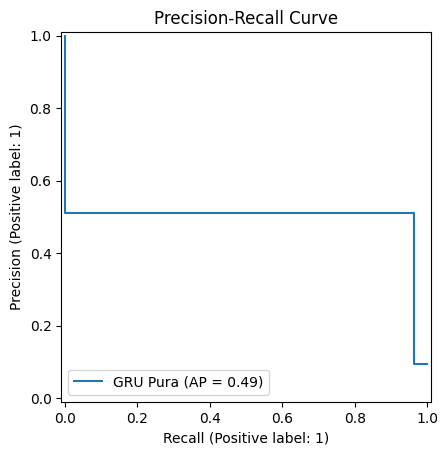
\includegraphics[width=0.7\textwidth]{figuras/modelos_resultados/ap_gru_pior_fold.png} % insere o tikzpicture puro
  \caption{Curva precisão vs \textit{recall} do modelo \ref{fig:gru_pura} em seu melhor \textit{fold}}
  \label{fig:ap_gru_pior_fold}
\end{figure}

Nesse gráfico, o \textit{baseline} não é fixo, mas igual a prevalência da classe positivos. No pior \textit{fold}, a proporção foi de aproximadamente
9,39\%, contrastando com o 49\% alcançado pelo modelo. Entretanto, a precisão foi baixa, pelo gráfico, é possível ver que, por exemplo, seria 
possível ter um recall de 80\% porém com uma precisão menor que 60\%.

No melhor caso:

\begin{figure}[H]
  \centering
   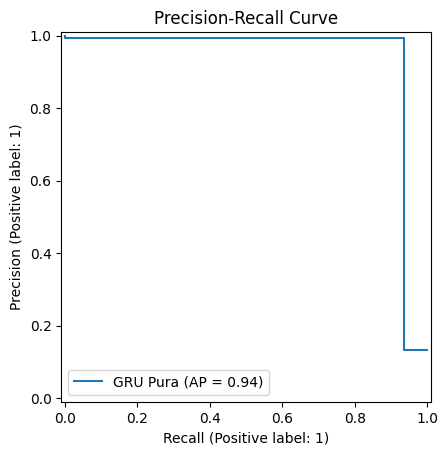
\includegraphics[width=0.7\textwidth]{figuras/modelos_resultados/ap_gru_melhor_fold.png} % insere o tikzpicture puro
  \caption{Curva precisão vs \textit{recall} do modelo \ref{fig:gru_pura} em seu melhor \textit{fold}}
  \label{fig:ap_gru_melhor_fold}
\end{figure}

Nesse \textit{fold}, o modelo alcançou um \textit{AP} de 80\%, enquanto que a proporção de casos positivos foi de 13,21\%. No melhor caso, 
entretanto, o modelo para ter 80\% de \textit{recall}, teria que baixar sua precisão para menos de 20\%. 

Apesar do desbalanceamento, o modelo alcançou resultados satisfatórios, considerando o extremo desbalanceamento do conjunto.

\chapter{Conclusão}

Texto da conclusão.

% Referências (BibTeX)
\bibliographystyle{abntex2-alf}
\bibliography{referencias}

\end{document}
